\documentclass[11pt]{amsart}

\usepackage{url,amsmath,mathtools,bbm,amsthm}
\usepackage[margin=1.15in]{geometry}

\newcommand{\E}{\mathbbm{E}}
\newcommand{\R}{\mathbbm{R}}
\newcommand{\N}{\mathbbm{N}}
\newcommand{\mathd}{\mathrm{d}}
\newcommand{\dx}[1]{\,\mathd #1}

\newtheorem{theorem}{Theorem}

\begin{document}

\title{Homework 0: Basics of submission\\MATH 6610-001, Fall 2019}
\author{Akil Narayan}
\maketitle

The topic of this homework assignment is usage of Monte Carlo techniques to approximate the transcendental number $\pi$.  The setup is as follows: let $\rho : [-1,1]^2 \rightarrow \R$ be the uniform probability density on the square $[-1,1]^2 \subset \R^2$. I.e, $\rho(x,y) = 1/4$ if both $x$ and $y$ satisfy $|x| < 1$ and $|y| < 1$, and $\rho$ is zero otherwise. We consider the function $f$ that is the indicator of the unit ball in $\R^2$ centered at the origin:
\begin{align*}
  f(x) &= \mathbbm{1}_R(x) = \left\{ \begin{array}{rl} 1, & x \in R, \\ 0, & x \not\in R \end{array}\right.,
       & 
     R &\coloneqq \left\{ (x_1, x_2) \in \R^2\, \big|\, x_1^2 + x_2^2 \leq 1 \right\}.
\end{align*}
Note then that 
Now let $X \in \R^2$ be a random variable whose probability density is $\rho$. We have,
\begin{align*}
  4 \E f(X) = 4 \int_{[-1,1]^2} f(x) \frac{1}{4} \dx{x} \dx{y} = \pi.
\end{align*}
We seek to build a computational estimator to $4 \E f(X)$, which should approximate $\pi$. Given a fixed $M \in \N$, define $F_M$ as:
\begin{align}\label{eq:FM-def}
  4 F_M \coloneqq \frac{4}{M} \sum_{m=1}^M f(X_m),
\end{align}
where $\{X_m\}_{m=1}^M$ are independent and identically distributed copies of $X$. We can compute realizations of $4 F_M$ simply by generating uniformly distributed random numbers on $[-1,1]^2$ and evaluating $f$. We expect that larger $M$ yields a better approximation.

To investigate the quality of this approximation, we compute statistics for the random variable $\left| 4 F_M - \pi \right|$. Figure \ref{fig:FM} shows the results over a fairly large range for $M$, where 10\% and 90\% quantiles along with the median are shown. The results indicate that, indeed, as $M$ is increased the random variable $4 F_M$ concentrates more around $\pi$, and hence $4 F_M$ becomes a statistically better approximation to $\pi$ for large $M$. 

\begin{figure}[htbp]
  \begin{center}
    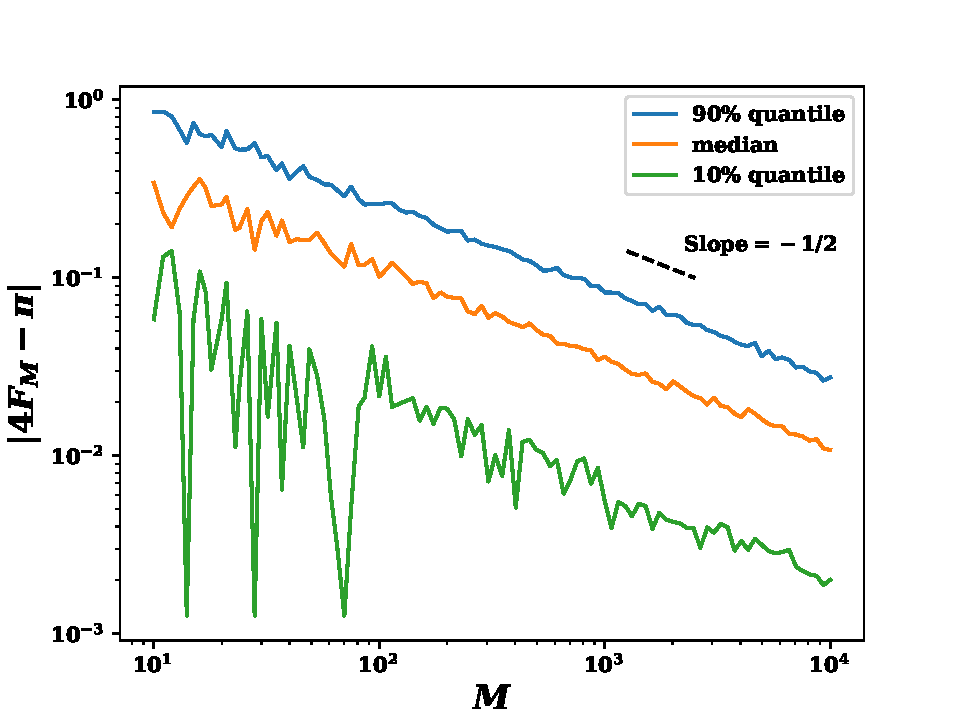
\includegraphics[width=0.5\textwidth]{FM_stats.pdf}
  \end{center}
  \caption{Quantiles (10\%, 90\%) and median for the random variable $\left| 4 F_M - \pi \right|$ as a function of $M$. Also plotted is a curve corresponding to $1/\sqrt{M}$.}\label{fig:FM}
\end{figure}

Our next task is to verify the Central Limit Theorem (CLT) using samples from $F_M$. Before doing this, we state the CLT.
\begin{theorem}[Central Limit Theorem]
  Let $\{Y_j\}_{j \geq 1}$ be independent and identically distributed random variables with finite mean and variance, $\E Y_j = \mu$ and $\mathrm{Var} Y_j = \sigma^2$. Define $S_M$ as the normalized sum of the first $M$ copies of $Y_j$:
  \begin{align*}
    S_M \coloneqq \frac{1}{M} \sum_{j=1}^M Y_j.
  \end{align*}
  Then $S_M$ converges in distribution to a normally-distributed random variable. More precisely:
  \begin{align*}
    \lim_{M \rightarrow \infty} \frac{\sqrt{M}}{\sigma} \left( S_M - \mu \right) = \mathcal{N}(0, 1),
  \end{align*}
  where $\mathcal{N}(0,1)$ means a random variable with the standard normal distribution, and the equality is in distribution.
\end{theorem}
We will verify this theorem by comparing histograms for an ensemble (of a translated and scaled version) of $F_M$ to the predicted density given by the CLT. Precisely, since from \eqref{eq:FM-def} we have
\begin{align*}
  F_M = \frac{1}{M} \sum_{m=1}^M f(X_m),
\end{align*}
then the CLT states that 
\begin{align*}
  G_M \coloneqq \frac{\sqrt{M}}{\sigma_f} \left(F_M - \mu_f\right) 
\end{align*}
converges in distribution to a standard normal random variable as $M \uparrow \infty$. Above $\mu_f$ and $\sigma_f$ are the mean and standard deviation of $f(X)$, respectively. These can be computed:
\begin{align*}
  \mu_f &= \E f(X) = \frac{\pi}{4} \\
  \sigma^2_f &= \E\left[ f(X)^2\right] - \left( \E f(X)\right)^2 = \frac{\pi}{4} - \left(\frac{\pi}{4}\right)^2
\end{align*}
where we have used the fact that $\mathrm{Var}(Y) = \E Y^2 - (\E Y)^2$, and that $f(X)^2 = f(X)$. With all these quantities computed, we can now test, via histograms, whether $G_M$ behaves like a standard normal random variable for large $M$. The density of a standard normal random variable is
\begin{align*}
  \varphi(x) = \frac{1}{\sqrt{2 \pi}} \exp(-x^2/2),
\end{align*}
so that we can visually compare (normalized) histograms of $G_M$ against this function. Figure \ref{fig:CLT} shows these comparisons for three values of $M$. As $M$ is increased, the histograms visually begin to represent $\varphi(x)$ more. This verifies, at least qualitatively, that the Central Limit Theorem holds for this simulation.
\begin{figure}
  \begin{center}
    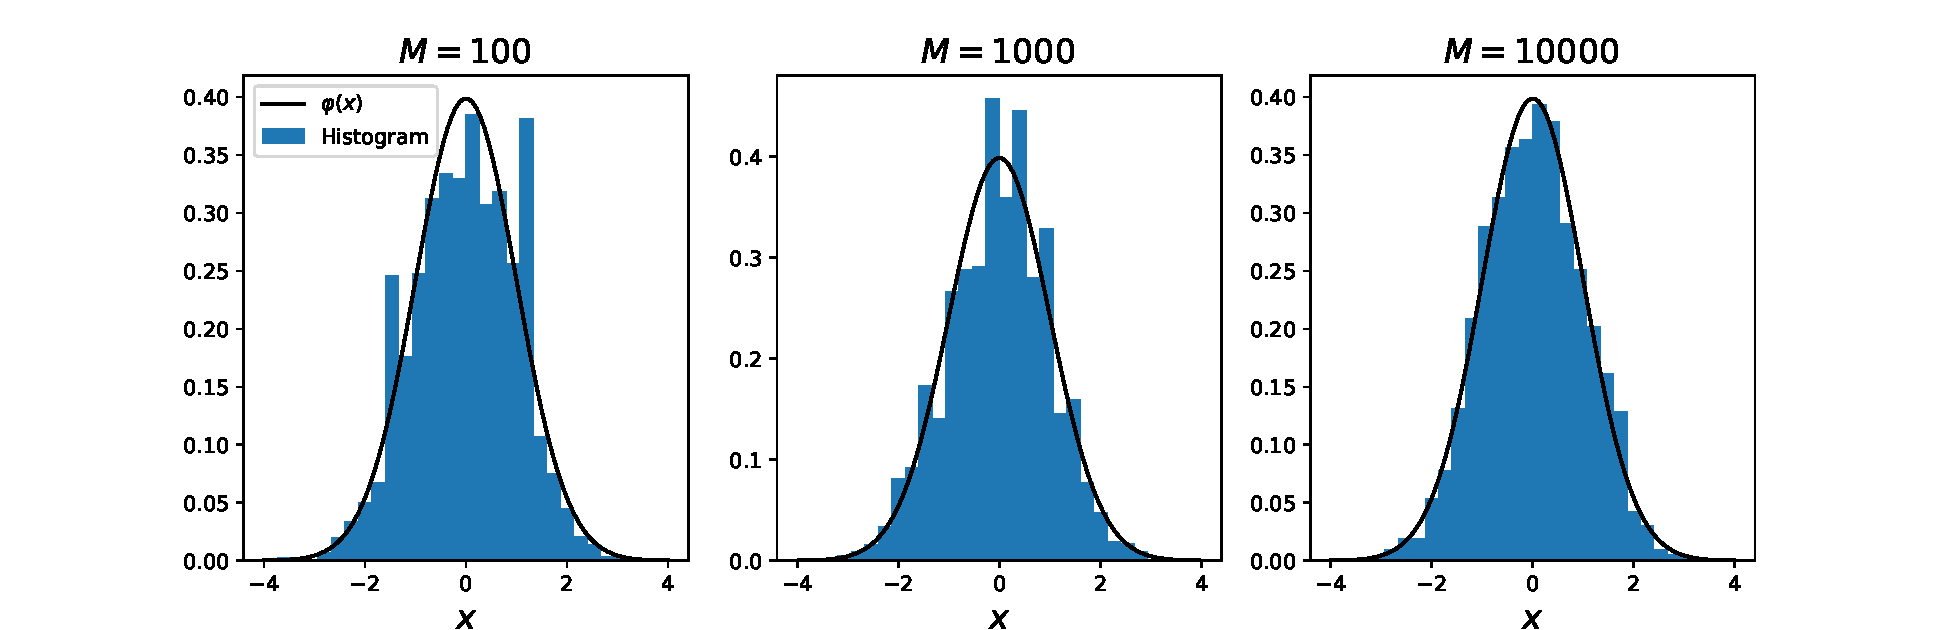
\includegraphics[width=\textwidth]{CLT.pdf}
  \end{center}
  \caption{Normalized histograms of 3000 realizations of $G_M$ versus the CLT-predicted large-$M$ behavior $\varphi(x)$. Left, center, and right: $M = 10^2, 10^3$, and $10^4$, respectively.}\label{fig:CLT}
\end{figure}

\end{document}
